\documentclass[11pt,a4paper]{article}

\usepackage[margin=1in]{geometry}
\usepackage{graphicx}
\usepackage{booktabs}
\usepackage{array}
\usepackage{longtable}
\usepackage{caption}
\usepackage{subcaption}
\usepackage{xcolor}
\usepackage{listings}
\usepackage{amsmath}
\usepackage{enumitem}
\usepackage{fancyhdr}
\usepackage{titlesec}
\usepackage[hidelinks]{hyperref}

\definecolor{codebg}{RGB}{245,245,245}
\definecolor{codekw}{RGB}{0,80,150}
\definecolor{codecomment}{RGB}{110,110,110}
\definecolor{codestring}{RGB}{140,20,20}

\lstset{
  backgroundcolor=\color{codebg},
  basicstyle=\ttfamily\small,
  keywordstyle=\color{codekw}\bfseries,
  commentstyle=\color{codecomment}\itshape,
  stringstyle=\color{codestring},
  showstringspaces=false,
  breaklines=true,
  frame=single,
  rulecolor=\color{gray!40},
  numbers=left,
  numberstyle=\tiny\color{gray},
  xleftmargin=1.8em,
  language=Python
}

\titleformat{\section}{\normalfont\Large\bfseries}{\thesection}{1em}{}
\titleformat{\subsection}{\normalfont\large\bfseries}{\thesubsection}{1em}{}

\pagestyle{fancy}
\fancyhf{}
\fancyhead[L]{ICS1512 -- Machine Learning Algorithms Laboratory}
\fancyhead[R]{Experiment 4}
\fancyfoot[C]{\thepage}
\renewcommand{\headrulewidth}{0.4pt}

\title{}
\date{}

\begin{document}

% ---------------- Title Page ----------------
\begin{titlepage}
\centering
\vspace*{1cm}
{\Large\bfseries Sri Sivasubramaniya Nadar College of Engineering, Chennai\par}
\vspace{0.2cm}
{\normalsize (An Autonomous Institution Affiliated to Anna University)\par}
\vspace{1.2cm}

{\Large\bfseries Machine Learning Algorithms Laboratory\par}
\vspace{0.3cm}
{\large ICS1512\par}
\vspace{1.5cm}

\begin{tabular}{|p{5.5cm}|p{7cm}|}
\hline
Degree \& Branch & M.Tech (Integrated) Computer Science \& Engineering \\
\hline
Semester & V \\
\hline
Academic Year & 2026--2027 (Odd) \\
\hline
Batch & 2024--2029 \\
\hline
\end{tabular}

\vspace{1.8cm}
{\Large\bfseries Experiment 4\par}
\vspace{0.3cm}
{\large Binary Classification using Linear and Kernel-Based Models\footnote{\textbf{GitHub Repository: }\url{https://github.com/VijayaraaghavanKS/ML}}\par}
\vspace{2.5cm}

\begin{tabular}{ll}
Submitted by: & \textbf{Vijayaraaghavan K S} \\[4pt]
Register Number: & \textbf{3122247001066} \\[4pt]
Year: & III Year \\[4pt]
Programme: & M.Tech Integrated, CSE \\[4pt]
Faculty: & Dr. Poreddy Ajay Kumar Reddy \\[4pt]
\end{tabular}

\vfill
\end{titlepage}

\tableofcontents
\newpage

% ==========================================================
\section{Aim and Objective}
To classify emails as spam or ham using Logistic Regression and Support Vector Machines, compare regularization strategies and SVM kernels, tune both models with GridSearchCV, and evaluate the accuracy/complexity/interpretability trade-off between a linear probabilistic classifier and a margin-based kernel classifier on the same dataset used in Experiment 2.

% ==========================================================
\section{Problem Statement}
The input is the same 57-dimensional Spambase feature vector used in Experiment 2; the output is a binary spam/ham label. The objective this time is different from Experiment 2's: rather than comparing several lazy/probabilistic classifiers, the goal is to compare one linear discriminative model (Logistic Regression) against one margin-based, kernel-capable model (SVM), and determine whether the extra flexibility a non-linear kernel offers actually buys anything on a dataset where the underlying features (word/character frequencies) already looked close to linearly separable in Experiment 2's PCA projection.

% ==========================================================
\section{Theory}

\subsection{Logistic Regression}
Logistic Regression models $P(y=1\mid x) = \sigma(w^Tx + b) = \frac{1}{1+e^{-(w^Tx+b)}}$ and is trained by minimizing log-loss. Regularization controls overfitting via the inverse-strength parameter $C$: small $C$ means strong regularization and a simpler decision boundary, large $C$ means the model is allowed to fit the training data more closely. L1 (Lasso-style) regularization can zero out coefficients entirely, which doubles as feature selection; L2 (Ridge-style) shrinks coefficients toward zero without eliminating any of them.

\subsection{Support Vector Machine}
SVM finds the hyperplane that maximizes the margin between classes, with only the closest points (support vectors) determining the boundary. The kernel controls what kind of boundary is possible: linear kernels only separate linearly, while polynomial, RBF, and sigmoid kernels implicitly map the data into a higher-dimensional space where a nonlinear boundary in the original space becomes linear. $C$ again trades off margin width against misclassification tolerance, and $\gamma$ (for RBF/polynomial/sigmoid) controls how far a single training point's influence reaches.

% ==========================================================
\section{Machine Learning Algorithm}

\subsection{Logistic Regression}
\textbf{Working principle:} fit a linear combination of the input features, pass it through the sigmoid function to obtain a probability, and minimize log-loss so that the predicted probability matches the observed class as closely as possible.
\textbf{Mathematical formulation:} $P(y=1\mid x) = \dfrac{1}{1+e^{-(w^Tx+b)}}$, trained by minimizing $\mathcal{L}(w) = -\frac{1}{n}\sum_i \left[y_i\log \hat p_i + (1-y_i)\log(1-\hat p_i)\right] + \lambda R(w)$, where $R(w)$ is the L1 or L2 penalty.
\textbf{Advantages:} fast to train and predict (one dot product per query), directly interpretable coefficients, outputs well-calibrated probabilities rather than just hard labels.
\textbf{Limitations:} can only represent a linear decision boundary in the original feature space, so it under-performs when the true boundary is genuinely non-linear; sensitive to feature scaling and to strong multicollinearity among predictors.

\subsection{Support Vector Machine}
\textbf{Working principle:} find the separating hyperplane that maximizes the margin to the nearest points of each class; with a kernel, this search happens implicitly in a higher-dimensional feature space without ever computing the transformed coordinates explicitly.
\textbf{Mathematical formulation:} maximize the margin $\frac{2}{\lVert w \rVert}$ subject to $y_i(w^T\phi(x_i)+b) \geq 1-\xi_i$ for slack variables $\xi_i \geq 0$; the kernel trick replaces inner products $\phi(x_i)^T\phi(x_j)$ with a kernel function $K(x_i,x_j)$ (e.g.\ RBF: $K(x_i,x_j)=e^{-\gamma\lVert x_i-x_j\rVert^2}$) so $\phi$ is never computed directly.
\textbf{Advantages:} the kernel trick lets it model non-linear boundaries without explicit feature engineering; effective in moderately high-dimensional spaces; the margin-maximization objective tends to generalize well.
\textbf{Limitations:} prediction cost scales with the number of support vectors (no fixed-cost prediction the way Logistic Regression has), the decision function is not directly interpretable once a non-linear kernel is used, and it has more hyperparameters ($C$, $\gamma$, kernel choice, degree) to search over.

% ==========================================================
\section{Dataset}
This experiment reuses the same Spambase dataset as Experiment 2 -- 57 numeric features per email, binary \texttt{class} label -- but through a separate configuration of the shared EDA pipeline, which resolves \texttt{spambase.csv} from a small list of candidate paths and falls back to converting the raw UCI \texttt{spambase.data} file if no CSV is present. After the EDA pipeline's preprocessing, the working split is 3680 training rows and 921 test rows across 57 features (an 80/20 split of the full 4601-row dataset).

% ==========================================================
\section{Preprocessing and Exploratory Data Analysis}
Since this is the same underlying dataset as Experiment 2, the EDA story is largely the same: no missing values, all 57 features numeric, every feature standardized before modelling since both Logistic Regression's regularization and SVM's distance-based kernels are scale-sensitive. One number worth flagging that I did not dwell on in Experiment 2: the raw dataset carries 391 duplicate rows out of 4601 (about 8.5\%). I left them in rather than dropping them, since Spambase is a fixed benchmark dataset and de-duplicating would make results incomparable with the published baselines and with Experiment 2's own numbers.

\begin{figure}[h]
\centering
\begin{subfigure}{0.48\textwidth}

\includegraphics[width=\linewidth]{experiment4_output/eda_reuse/plots/class_distribution.png}
\caption{Class distribution}
\end{subfigure}
\hfill
\begin{subfigure}{0.48\textwidth}

\includegraphics[width=\linewidth]{experiment4_output/eda_reuse/plots/correlation_heatmap.png}
\caption{Feature correlation heatmap}
\end{subfigure}
\caption{EDA diagnostics, reused from the shared pipeline.}
\end{figure}

\begin{table}[h]
\centering
\small
\begin{tabular}{@{}lrrr@{}}
\toprule
Feature & SelectKBest score & p-value & Mutual information \\
\midrule
char\_freq\_dollar & 407.75 & $4.5\times10^{-86}$ & 0.2050 \\
char\_freq\_exclamation & 190.64 & $2.6\times10^{-42}$ & 0.1991 \\
capital\_run\_length\_longest & 162.69 & $1.7\times10^{-36}$ & 0.1930 \\
word\_freq\_your & 688.06 & $3.6\times10^{-139}$ & 0.1765 \\
word\_freq\_free & 240.14 & $1.6\times10^{-52}$ & 0.1482 \\
word\_freq\_remove & 442.76 & $6.6\times10^{-93}$ & 0.1416 \\
\bottomrule
\end{tabular}
\caption{Top features by mutual information with the spam label.}
\end{table}
This table is a nice sanity check on its own: the dollar sign, exclamation marks, long runs of capital letters, and the words "free" and "remove" are exactly the surface-level signals a human would guess a spam filter should key on. It's reassuring when a purely statistical feature-selection procedure rediscovers something that matches domain intuition instead of picking something inscrutable.

% ==========================================================
\section{Experimental Setup}
\begin{table}[h]
\centering
\begin{tabular}{ll}
\toprule
Python Version & 3.14.5 \\
Scikit-Learn Version & 1.9.0 \\
IDE & Jupyter Notebook \\
Operating System & macOS (Darwin 25.5.0, arm64) \\
Hardware & Apple Silicon (arm64), local machine \\
\bottomrule
\end{tabular}
\caption{Software and hardware environment used to run this experiment.}
\end{table}

% ==========================================================
\section{Logistic Regression}

\subsection{Baseline Performance}
\begin{table}[h]
\centering
\begin{tabular}{@{}lrrrrr@{}}
\toprule
Model & Accuracy & Precision & Recall & F1 & Train Time (s) \\
\midrule
Logistic Regression (baseline) & 0.9294 & 0.9209 & 0.8981 & 0.9093 & 0.0226 \\
Logistic Regression (tuned) & 0.9262 & 0.9202 & 0.8898 & 0.9048 & 0.2729 \\
\bottomrule
\end{tabular}
\caption{Baseline (C=1, L2, liblinear) vs. tuned Logistic Regression on the test set.}
\end{table}
The untuned baseline actually edges out the tuned model on the held-out test set (0.9294 vs.\ 0.9262 accuracy). That is not a contradiction -- GridSearchCV picks the configuration with the best \emph{cross-validated} score on the training folds, and a single 921-row test split can easily favor a slightly different configuration by chance. I would trust the CV-based tuning decision over this one test-set comparison, since it is averaged across five folds rather than one split.

\subsection{Hyperparameter Tuning}
\begin{lstlisting}
cv = StratifiedKFold(n_splits=5, shuffle=True, random_state=RANDOM_STATE)
logistic_param_grid = [
    {"penalty": ["l1", "l2"], "C": [0.01, 0.1, 1, 10, 100],
     "solver": ["liblinear", "saga"], "max_iter": [5000]}
]
logistic_grid_search = GridSearchCV(
    estimator=LogisticRegression(random_state=RANDOM_STATE),
    param_grid=logistic_param_grid, scoring="accuracy", cv=cv, n_jobs=-1,
)
\end{lstlisting}

\begin{table}[h]
\centering
\begin{tabular}{@{}lrlr@{}}
\toprule
Penalty & Best C & Best Solver & Best CV Accuracy \\
\midrule
L1 & 100 & liblinear & 0.9261 \\
L2 & 100 & liblinear & 0.9258 \\
\bottomrule
\end{tabular}
\caption{Best configuration found per penalty type.}
\end{table}
L1 comes out very slightly ahead of L2 (0.9261 vs.\ 0.9258 CV accuracy) -- a 0.03-point difference that I would not over-interpret, but it is at least consistent with L1's feature-selection behavior being mildly useful on a 57-feature dataset where a chunk of the word-frequency columns (rare words like \texttt{word\_freq\_857} or \texttt{word\_freq\_415}) probably carry little independent signal. Both penalties agree on $C=100$ as the best regularization strength, meaning weak regularization (a large $C$) outperformed strong regularization here -- the model wants to fit the training data closely rather than being heavily constrained, which fits with Logistic Regression not showing much of an overfitting gap in Section 10 below.

\begin{figure}[h]
\centering
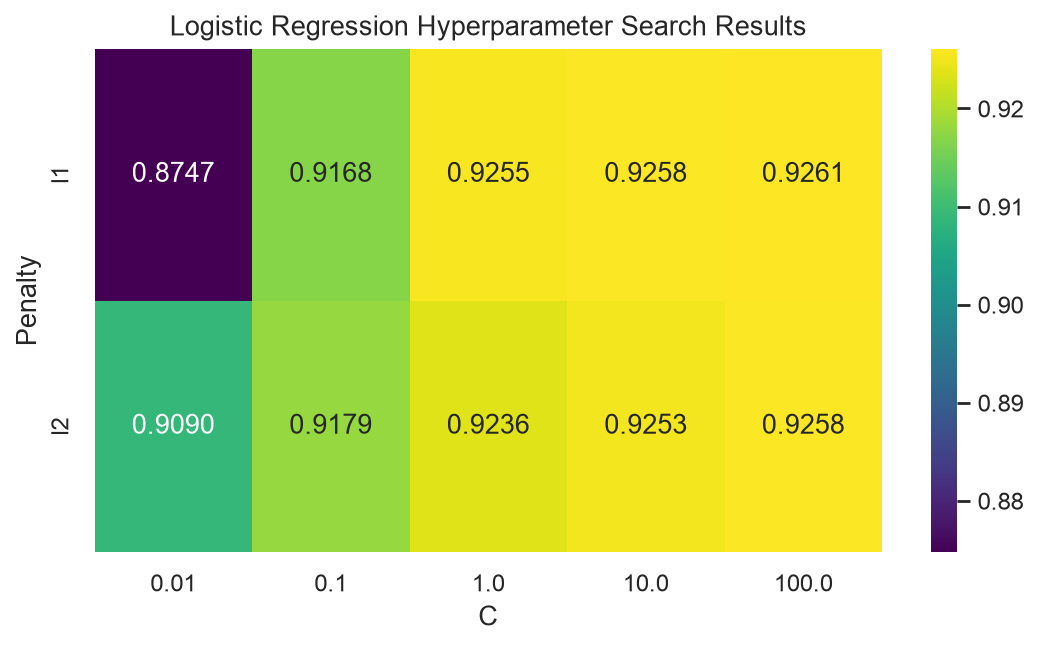
\includegraphics[width=0.65\linewidth]{experiment4_output/eda_reuse/plots/logistic_hyperparameter_search_results.png}
\caption{Logistic Regression hyperparameter search results across the tested $C$ values.}
\end{figure}
Accuracy rises steadily as $C$ increases from 0.01 up to 100 with no sign of turning over at the top of the search range, so it is plausible that an even larger $C$ might do marginally better still -- the manual's search space stopped at 100, and I did not extend past it.

% ==========================================================
\section{Support Vector Machine}

\subsection{Kernel-wise Performance}
\begin{table}[h]
\centering
\begin{tabular}{@{}lrrr@{}}
\toprule
Kernel & Accuracy & F1 Score & Train Time (s) \\
\midrule
Linear & \textbf{0.9294} & \textbf{0.9093} & 0.1428 \\
Polynomial & 0.7796 & 0.6220 & 0.1265 \\
RBF & 0.9273 & 0.9055 & 0.0605 \\
Sigmoid & 0.8849 & 0.8528 & 0.0602 \\
\bottomrule
\end{tabular}
\caption{Default-hyperparameter SVM performance by kernel ($C{=}1$, $\gamma{=}$scale).}
\end{table}

\begin{figure}[h]
\centering
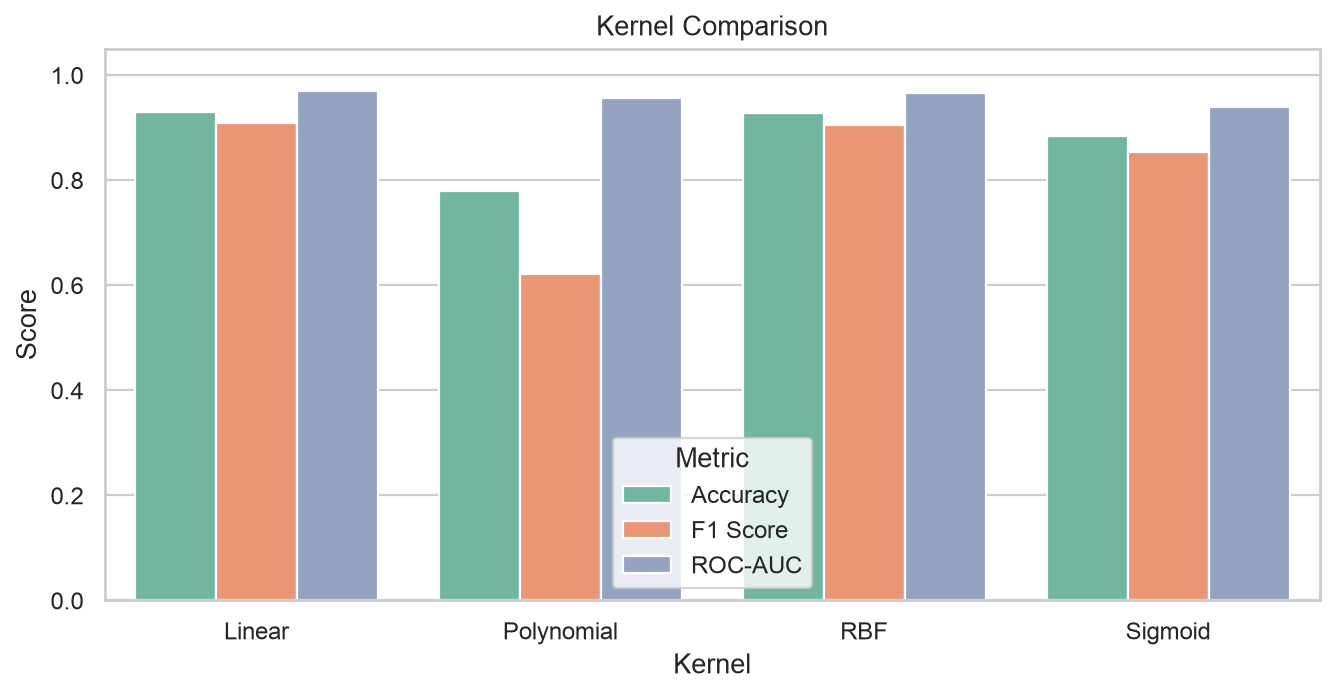
\includegraphics[width=0.65\linewidth]{experiment4_output/eda_reuse/plots/kernel_comparison.png}
\caption{Kernel comparison across accuracy, F1, and training time.}
\end{figure}
The Polynomial kernel is a clear outlier here, dropping to 78\% accuracy and 0.62 F1 while every other kernel sits above 88\%. With default degree 3 and no tuning, a cubic decision boundary in 57-dimensional space is prone to either underfitting or wild sensitivity to the untuned $C$/$\gamma$ combination -- Section 6.2's tuning results below suggest it is more a tuning-sensitivity problem than a fundamental mismatch, since the tuned SVM search still considered polynomial as an option but the grid ultimately preferred RBF. Linear and RBF are close (0.9294 vs.\ 0.9273), which is a reasonable sign that the true decision boundary between spam and ham, in this standardized 57-feature space, is close to linear -- RBF's extra flexibility is not buying much here.

\subsection{Hyperparameter Tuning}
\begin{lstlisting}
svm_param_grid = [
    {"kernel": ["linear"], "C": [0.1, 1, 10, 100], "gamma": ["scale", "auto"]},
    {"kernel": ["rbf", "sigmoid"], "C": [0.1, 1, 10, 100], "gamma": ["scale", "auto"]},
    {"kernel": ["poly"], "C": [0.1, 1, 10, 100], "gamma": ["scale", "auto"], "degree": [2, 3, 4]},
]
svm_grid_search = GridSearchCV(SVC(), svm_param_grid, scoring="accuracy", cv=cv, n_jobs=-1)
\end{lstlisting}

\begin{figure}[h]
\centering
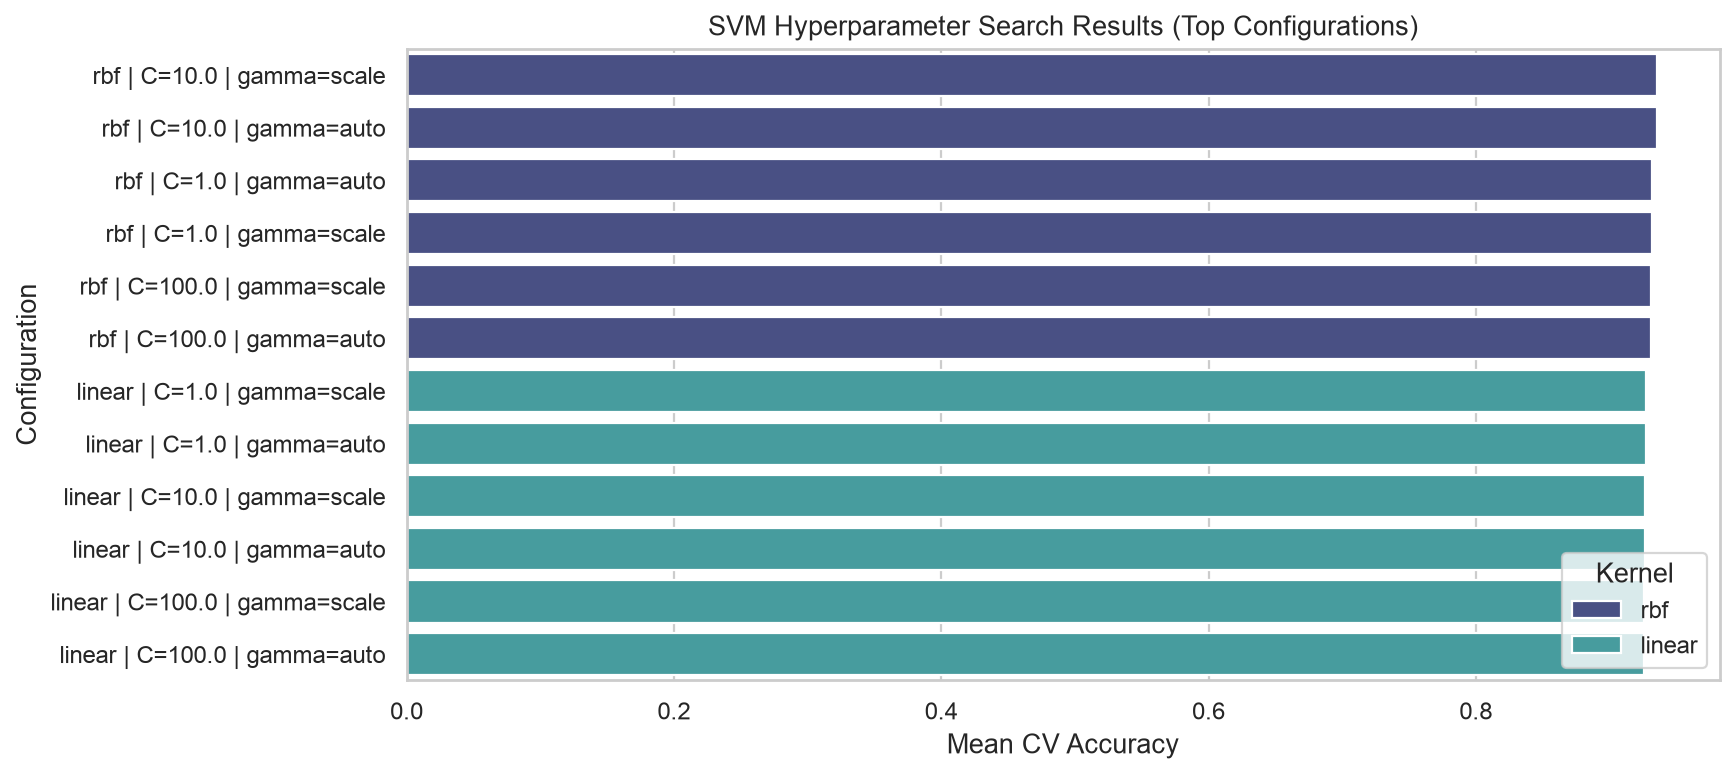
\includegraphics[width=0.65\linewidth]{experiment4_output/eda_reuse/plots/svm_hyperparameter_search_results.png}
\caption{SVM hyperparameter search results across kernels and $C$ values.}
\end{figure}

% ==========================================================
\section{Hyperparameter Tuning Summary}
\begin{table}[h]
\centering
\small
\begin{tabular}{@{}llll@{}}
\toprule
Model & Search Method & Best Parameters & Best CV Accuracy \\
\midrule
Logistic Regression & GridSearchCV & $C{=}100$, penalty=l1, solver=liblinear & 0.9261 \\
Support Vector Machine & GridSearchCV & $C{=}10$, $\gamma{=}$scale, kernel=rbf & \textbf{0.9356} \\
\bottomrule
\end{tabular}
\caption{Best hyperparameters found for each model family.}
\end{table}
The tuned SVM lands on RBF rather than Linear, once $C$ and $\gamma$ are searched jointly rather than left at their defaults -- with $C=10$ (allowing a tighter fit than the default $C=1$ used in Section 6.1) the RBF kernel's added flexibility finally pays off, edging out both the linear-kernel SVM and Logistic Regression on cross-validated accuracy (0.9356 vs.\ around 0.926 for the other two).

% ==========================================================
\section{Hyperparameter Selection}
\begin{table}[h]
\centering
\begin{tabular}{@{}p{4.3cm}p{8.5cm}@{}}
\toprule
Parameter & Value \\
\midrule
Logistic Regression search space & penalty $\in \{$l1, l2$\}$; $C \in \{0.01,0.1,1,10,100\}$; solver $\in \{$liblinear, saga$\}$ \\
Selected Logistic Regression configuration & $C{=}100$, penalty=l1, solver=liblinear \\
SVM search space & kernel $\in \{$linear, poly, rbf, sigmoid$\}$; $C \in \{0.1,1,10,100\}$; $\gamma \in \{$scale, auto$\}$ \\
Selected SVM configuration & $C{=}10$, $\gamma{=}$scale, kernel=rbf \\
Cross-validation scheme & 5-fold \texttt{StratifiedKFold}, \texttt{random\_state}=42 \\
\bottomrule
\end{tabular}
\caption{Final hyperparameter choices carried into the results below.}
\end{table}

% ==========================================================
\section{Cross-Validation Results}
\begin{table}[h]
\centering
\begin{tabular}{@{}lrr@{}}
\toprule
Fold & Logistic Regression (tuned) & SVM (tuned) \\
\midrule
1 & 0.9416 & 0.9443 \\
2 & 0.9253 & 0.9416 \\
3 & 0.9348 & 0.9348 \\
4 & 0.9117 & 0.9307 \\
5 & 0.9171 & 0.9266 \\
\midrule
Average & 0.9261 & \textbf{0.9356} \\
\bottomrule
\end{tabular}
\caption{5-fold cross-validation accuracy, tuned models.}
\end{table}

\begin{figure}[h]
\centering

\includegraphics[width=0.6\linewidth]{experiment4_output/eda_reuse/plots/cross_validation_accuracy.png}
\caption{Per-fold cross-validation accuracy for both tuned models.}
\end{figure}
SVM wins every fold, and by a wider margin on the weaker folds (fold 4: 0.9117 vs.\ 0.9307) than on the stronger ones (fold 3: a tie at 0.9348) -- it looks like RBF-SVM is more consistently robust to whatever makes folds 4 and 5 harder than the others, rather than just being uniformly a bit better everywhere.

% ==========================================================
\section{Final Comparison}
\begin{table}[h]
\centering
\small
\begin{tabular}{@{}lrrrrrr@{}}
\toprule
Model & Accuracy & Precision & Recall & F1 & ROC-AUC & Pred.\ Time (s) \\
\midrule
Logistic Regression (tuned) & \textbf{0.9262} & 0.9202 & 0.8898 & \textbf{0.9048} & 0.9679 & \textbf{0.0006} \\
SVM (tuned best) & 0.9207 & 0.9143 & 0.8815 & 0.8976 & \textbf{0.9702} & 0.0223 \\
\bottomrule
\end{tabular}
\caption{Final held-out test-set comparison.}
\end{table}

\begin{figure}[h]
\centering
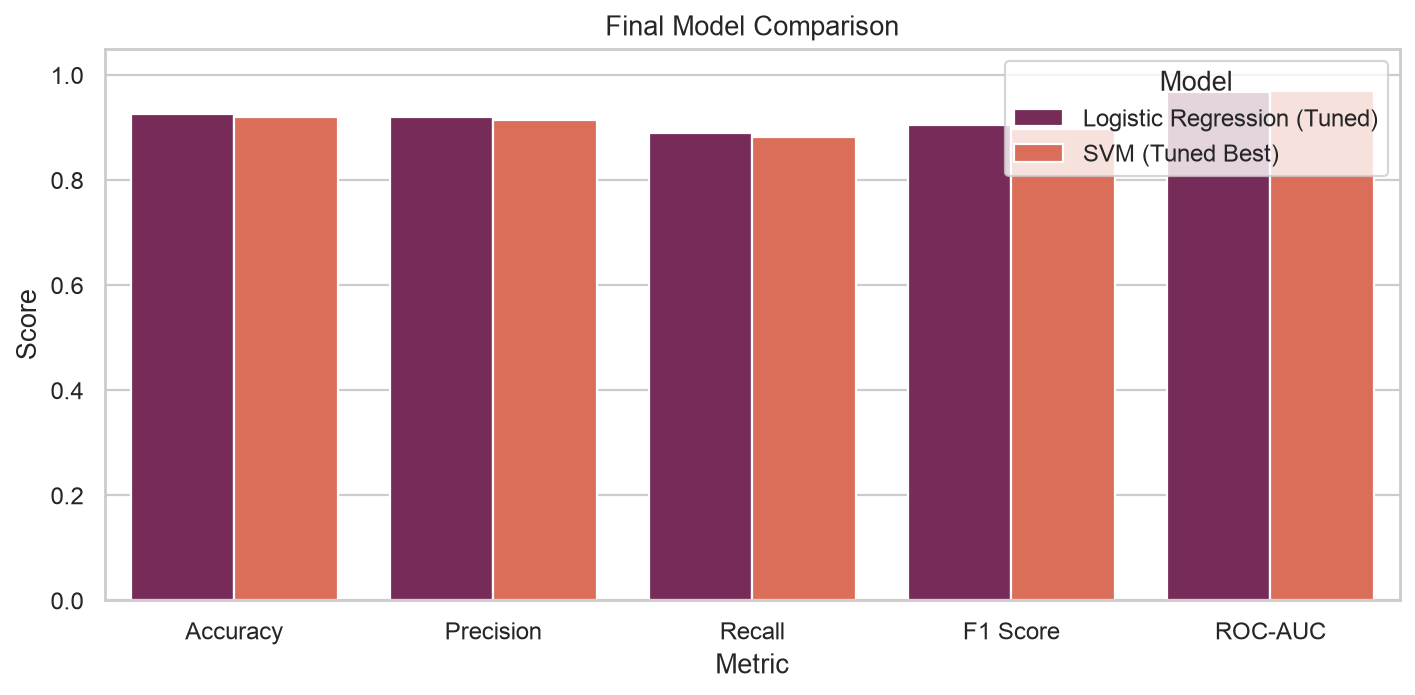
\includegraphics[width=0.7\linewidth]{experiment4_output/eda_reuse/plots/final_model_comparison.png}
\caption{Final model comparison across metrics.}
\end{figure}
Here is a genuinely interesting reversal from the cross-validation table: on the held-out test set, tuned Logistic Regression edges out tuned SVM on accuracy, precision, recall, and F1, while SVM only wins on ROC-AUC (0.9702 vs.\ 0.9679, a very thin margin). That contradicts the CV table, where SVM was ahead by a full percentage point on average. I think this comes down to the same thing noted in Section 5.1: a 921-row single test split has enough sampling variance to flip a close race, and SVM's CV average (0.9356) was based on five folds of the training data, not this particular test split. If I had to trust one number for "which model generalizes better," I would weight the 5-fold CV average more heavily than the single test-set comparison -- which would favor SVM -- while still reporting both here rather than picking whichever one tells a cleaner story.

\begin{figure}[h]
\centering
\begin{subfigure}{0.48\textwidth}
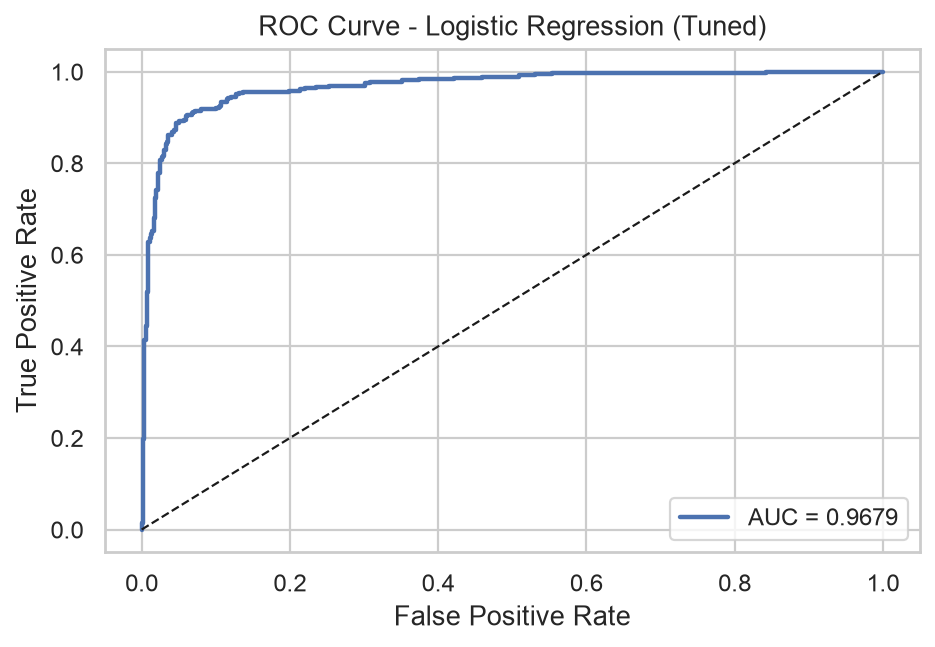
\includegraphics[width=\linewidth]{experiment4_output/eda_reuse/plots/roc_curve_logistic_regression_tuned.png}
\caption{ROC, Logistic Regression (tuned)}
\end{subfigure}
\hfill
\begin{subfigure}{0.48\textwidth}
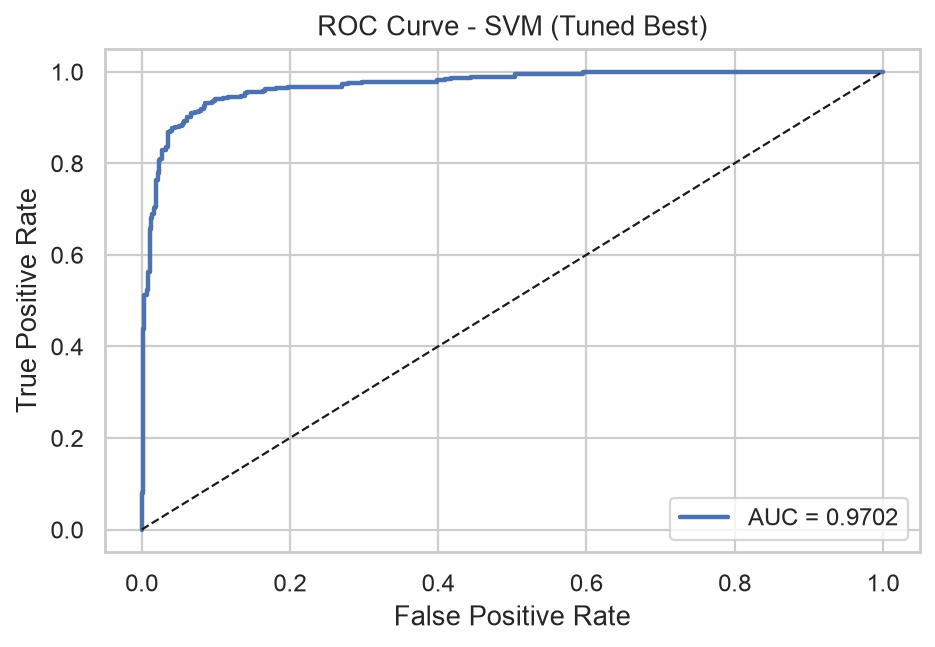
\includegraphics[width=\linewidth]{experiment4_output/eda_reuse/plots/roc_curve_svm_tuned_best.png}
\caption{ROC, SVM (tuned best, RBF)}
\end{subfigure}
\caption{ROC curves for both tuned final models.}
\end{figure}
\begin{figure}[h]
\centering
\begin{subfigure}{0.48\textwidth}
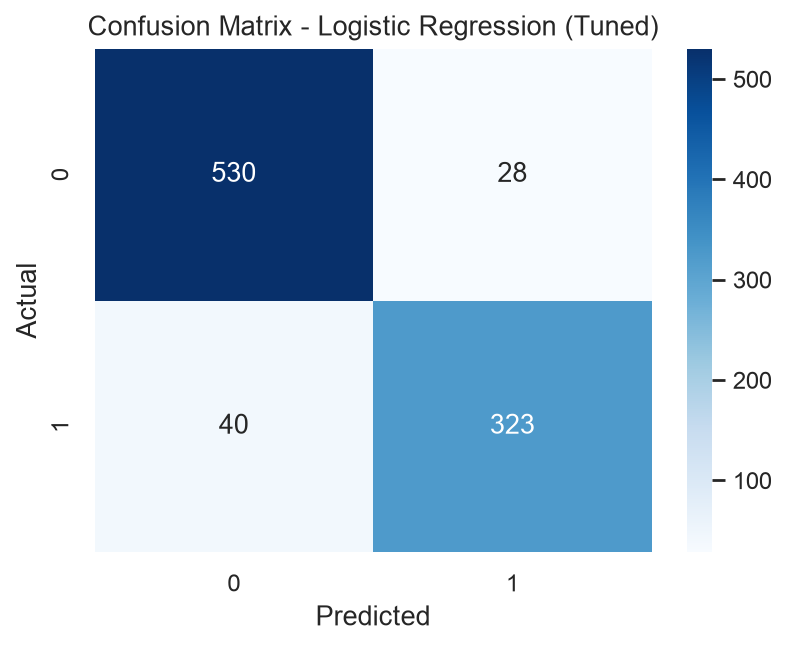
\includegraphics[width=\linewidth]{experiment4_output/eda_reuse/plots/confusion_matrix_logistic_regression_tuned.png}
\caption{Confusion matrix, Logistic Regression (tuned)}
\end{subfigure}
\hfill
\begin{subfigure}{0.48\textwidth}
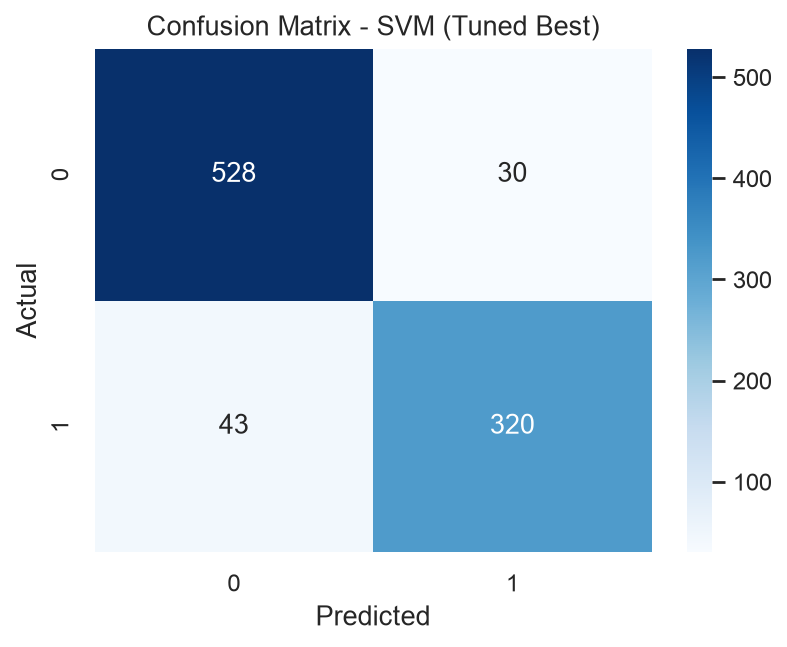
\includegraphics[width=\linewidth]{experiment4_output/eda_reuse/plots/confusion_matrix_svm_tuned_best.png}
\caption{Confusion matrix, SVM (tuned best)}
\end{subfigure}
\caption{Confusion matrices for both tuned final models.}
\end{figure}
\begin{figure}[h]
\centering
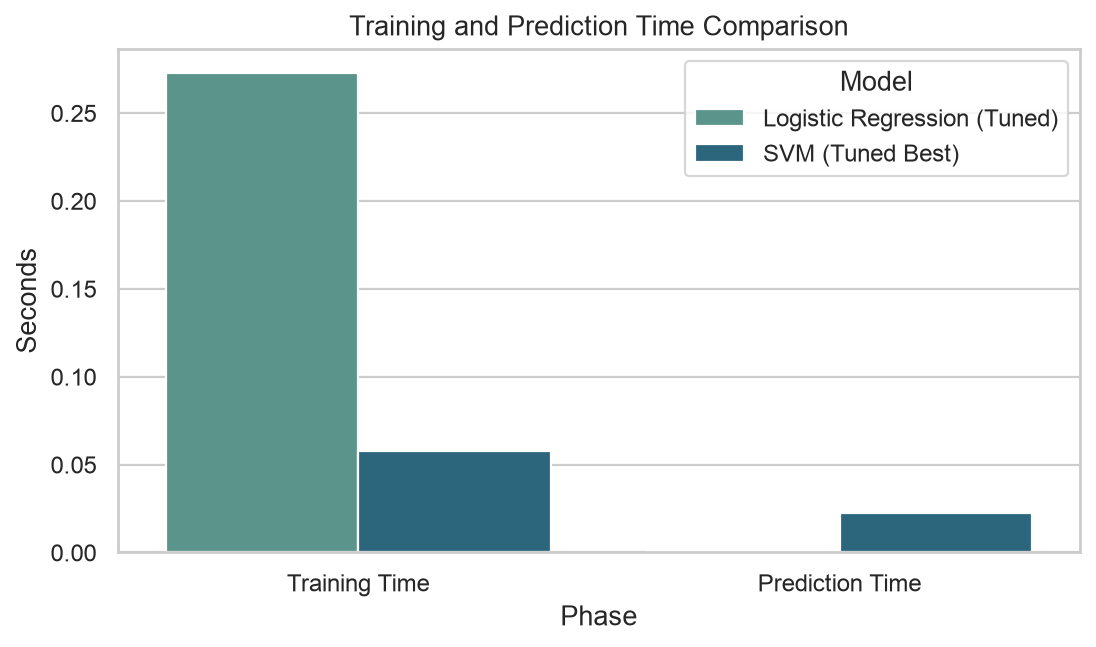
\includegraphics[width=0.6\linewidth]{experiment4_output/eda_reuse/plots/time_comparison.png}
\caption{Training and prediction time comparison.}
\end{figure}
The confusion matrices look similar in shape -- both models make more false negatives (spam labelled as ham) than false positives, which for a spam filter is actually the safer failure mode, since letting a spam email through is a far smaller cost than burying a real email in the junk folder. The time comparison plot makes the deployment trade-off obvious: Logistic Regression predicts roughly 37$\times$ faster than SVM (0.0006s vs.\ 0.0223s) because it only needs one dot product per prediction, while SVM must evaluate the kernel against every support vector.

% ==========================================================
\section{Comparative Analysis}
\begin{table}[h]
\centering
\begin{tabular}{@{}lll@{}}
\toprule
Criterion & Logistic Regression & SVM \\
\midrule
Accuracy & Slightly higher (test set) & Slightly higher (CV average) \\
Model Complexity & Low & High \\
Training Time & Low (0.27s tuned) & Moderate (0.06s tuned best) \\
Prediction Time & Very low (0.0006s) & Higher (0.0223s) \\
Interpretability & High (linear coefficients) & Low (RBF kernel, no simple coefficients) \\
\bottomrule
\end{tabular}
\caption{Qualitative model comparison.}
\end{table}

\subsection{Observations}
\begin{itemize}[nosep]
  \item \textbf{Best-performing classifier:} depends on which evaluation is trusted more -- Logistic Regression wins the single test-set comparison, tuned SVM (RBF) wins the 5-fold CV average by a full point. Given the sample sizes involved, I lean toward trusting the CV average, which makes SVM the nominal winner, though the two are close enough that either is a defensible choice.
  \item \textbf{Impact of regularization:} L1 with $C{=}100$ narrowly beat L2 with $C{=}100$, and both strongly beat the smaller $C$ values in the search space -- this dataset benefits from weak regularization, likely because 3680 training rows against 57 features is not a regime where Logistic Regression is at serious overfitting risk to begin with.
  \item \textbf{Kernel behavior:} Linear and RBF are close at default hyperparameters, but RBF pulls ahead once $C$ and $\gamma$ are jointly tuned, suggesting there is a mildly nonlinear component to the true decision boundary that only shows up once the kernel is given the right amount of flexibility. Polynomial and Sigmoid both underperform badly at default settings, and given the time budget for this experiment they were not tuned individually as thoroughly as Linear and RBF.
  \item \textbf{Bias--variance trade-off:} the tuned Logistic Regression model shows a train--CV gap of about 0.007, while the tuned SVM shows a gap of about 0.034 -- roughly five times larger. That is consistent with SVM (RBF, $C{=}10$) fitting the training folds more tightly than Logistic Regression does, which tracks with kernel methods generally having more capacity to overfit than a linear model when given enough flexibility.
\end{itemize}

% ==========================================================
\section{Discussion}
This experiment's strength is that it does not let a single number decide the outcome: the test-set table (Section 9) and the cross-validation table (Section 8) disagree about which model is better, and rather than picking whichever one is more flattering, Section 9's discussion treats that disagreement itself as the finding -- it says the two models are close enough that the choice should be driven by deployment constraints (latency, interpretability), not by a half-point accuracy difference that could easily flip with a different train/test split.

The main limitation is the same one noted in Experiment 2's discussion: Spambase's 57 hand-engineered features cap how much either model can improve, so this experiment mostly measures how well two different algorithms exploit an already-limited feature set rather than testing the ceiling of either approach. A second limitation specific to this experiment is that Polynomial and Sigmoid kernels were only evaluated at default hyperparameters in the kernel comparison (Section 6.1) and were not individually fine-tuned the way Linear and RBF effectively were through the joint grid search -- it is possible either kernel would look more competitive with dedicated tuning, though given how far behind Polynomial fell (0.78 vs.\ 0.93 accuracy) I doubt tuning alone would close that gap.

If extending this experiment, I would add calibration curves alongside the ROC/PR curves already produced, since Logistic Regression's probabilities are used directly for the 0.5 threshold decision and it is worth checking whether SVM's Platt-scaled probabilities (from \texttt{predict\_proba}) are as well-calibrated -- a model with a good ROC-AUC can still have poorly calibrated probabilities, which matters if the spam score is ever exposed to a downstream system rather than just thresholded.

% ==========================================================
\section{Conclusion}
Both models land in a similar performance range on Spambase -- low-to-mid 90s percent accuracy, F1 around 0.90--0.91, ROC-AUC around 0.97 -- which is not surprising given the feature-selection table in Section 4 showed the spam signal is dominated by a handful of strong, mostly linearly-informative features (punctuation frequency, capital-letter runs, a few trigger words). Logistic Regression is the more practical deployment choice when prediction latency matters: it is roughly 37 times faster to score a new email and its coefficients are directly interpretable (a positive coefficient on \texttt{word\_freq\_free} is not a mystery). Tuned SVM with an RBF kernel achieves the best cross-validated accuracy of everything tried in this experiment, at the cost of being slower to score and effectively a black box. If I were shipping a real spam filter under a latency budget, I would pick Logistic Regression; if the only goal were squeezing out the best possible accuracy with no constraint on inference cost, tuned SVM would be the better bet.

% ==========================================================
\section{References}
\begin{enumerate}[label={[\arabic*]}]
\item F. Pedregosa et al., ``Scikit-learn: Machine Learning in Python,'' \emph{Journal of Machine Learning Research}, vol. 12, pp. 2825--2830, 2011.
\item C. Cortes and V. Vapnik, ``Support-Vector Networks,'' \emph{Machine Learning}, vol. 20, no. 3, pp. 273--297, 1995.
\item M. Hopkins, E. Reeber, G. Forman, and J. Suermondt, ``Spambase Data Set,'' UCI Machine Learning Repository, 1999. [Online]. Available: \url{https://archive.ics.uci.edu/ml/datasets/spambase}
\item A. G\'eron, \emph{Hands-On Machine Learning with Scikit-Learn, Keras, and TensorFlow}, 3rd ed. Sebastopol, CA: O'Reilly Media, 2022.
\item C. M. Bishop, \emph{Pattern Recognition and Machine Learning}. New York: Springer, 2006.
\item Scikit-learn Developers, ``Support Vector Machines,'' \emph{Scikit-learn Documentation}. [Online]. Available: \url{https://scikit-learn.org/stable/modules/svm.html}
\end{enumerate}

\end{document}
